\documentclass[a4paper,12pt]{article}

%===================================================================================
% Paquetes
%-----------------------------------------------------------------------------------
\usepackage{amsmath}
\usepackage{float}
\usepackage{amsfonts}
\usepackage{amssymb}
\usepackage[utf8]{inputenc}
\usepackage{listings}
\usepackage[pdftex]{hyperref}
\usepackage{graphicx}

\usepackage{listings}
\usepackage{color}

\definecolor{dkgreen}{rgb}{0,0.6,0}
\definecolor{gray}{rgb}{0.5,0.5,0.5}
\definecolor{mauve}{rgb}{0.58,0,0.82}
\def\code#1{\texttt{#1}}

\lstset{frame=tb,
  language=Python,
  aboveskip=3mm,
  belowskip=3mm,
  showstringspaces=false,
  columns=flexible,
  basicstyle={\small\ttfamily},
  numbers=none,
  numberstyle=\tiny\color{gray},
  keywordstyle=\color{blue},
  commentstyle=\color{dkgreen},
  stringstyle=\color{mauve},
  breaklines=true,
  breakatwhitespace=true,
  tabsize=3
}

%-----------------------------------------------------------------------------------
% Configuración
%-----------------------------------------------------------------------------------
\hypersetup{colorlinks,%
	    citecolor=black,%
	    filecolor=black,%
	    linkcolor=black,%
	    urlcolor=blue}


\begin{document}

 

\title{ej6}

\begin{titlepage}
	\centering
	\vspace*{\fill}
	\vspace*{0.5cm}
	\huge\bfseries
	Modelo de Red Meta Poblacional\\
	\vspace*{2cm}
	Manual de Usuario\\
	\vspace*{\fill}
\end{titlepage}

\section*{Instrucciones de uso}
Al abrir la página se muestra primeramente una pequeña sección de ayuda (Fig.1) que describe los parámetros necesarios a rellenar para la simulación.

\begin{figure}[H]
	\centering
	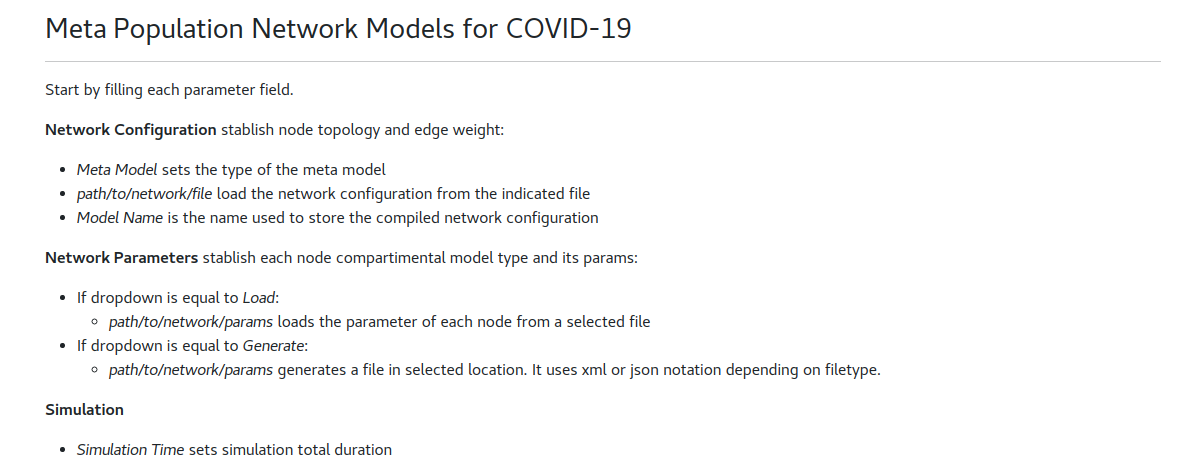
\includegraphics[width=0.9\linewidth]{./1}
	\caption{sección de ayuda}
	\label{Fig.1}
\end{figure}

A continuación se muestran los campos a rellenar (Fig.2)

\begin{figure}[H]
	\centering
	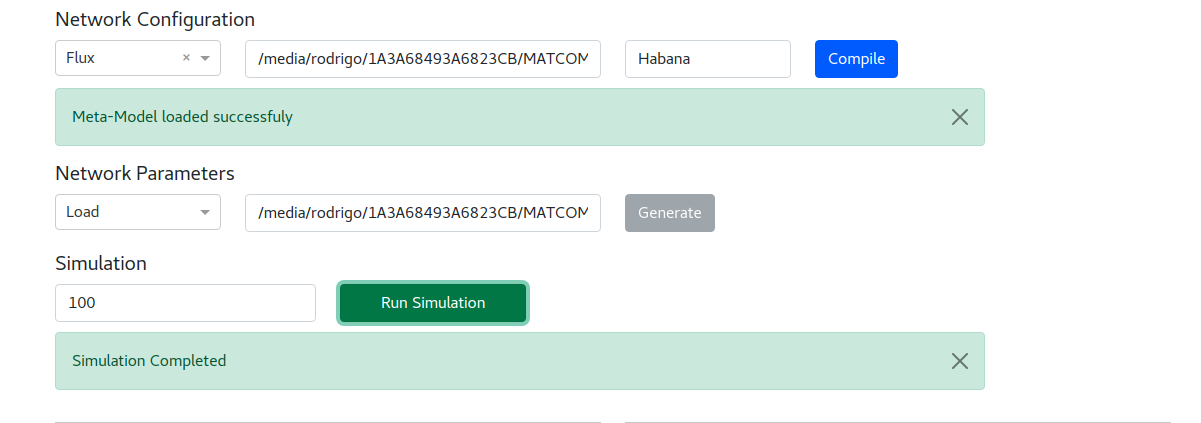
\includegraphics[width=0.9\linewidth]{./2}
	\caption{Campos de entrada}
	\label{Fig.2}
\end{figure}

Para la configuración de la red es necesario escoger el tipo de meta modelo e importar (poniendo la dirección local del archivo) una red preestablecida que puede ser de extensión .json o .xml (Más adelante se explica el formato que deben cumplir los archivos en cada caso). Luego de establecer un nombre, puede compilar la red.\\

Para importar los parámetros de los nodos, puede generar una plantilla o importar directamente una previamente generada.\\
 Para generar una plantilla de configuración de parámetros, seleccione la opción $Generate$ y proporcione una dirección destino. Una vez hecho esto, puede editar la plantilla con cualquier editor de texto para cambiar los parámetros convenientemente.\\
 Para cargar una configuración de parámetros seleccione la opción $Load$ y proporcione la direción del archivo en cuestión.\\
Independientemente del método de selección de parámetros utilizado, luego de establecer un tiempo de simulación, puede presionar el botón "Run Simulation" para iniciar la misma.\\

El resultado se muestra a continuación (Fig.3).

\begin{figure}[H]
	\centering
	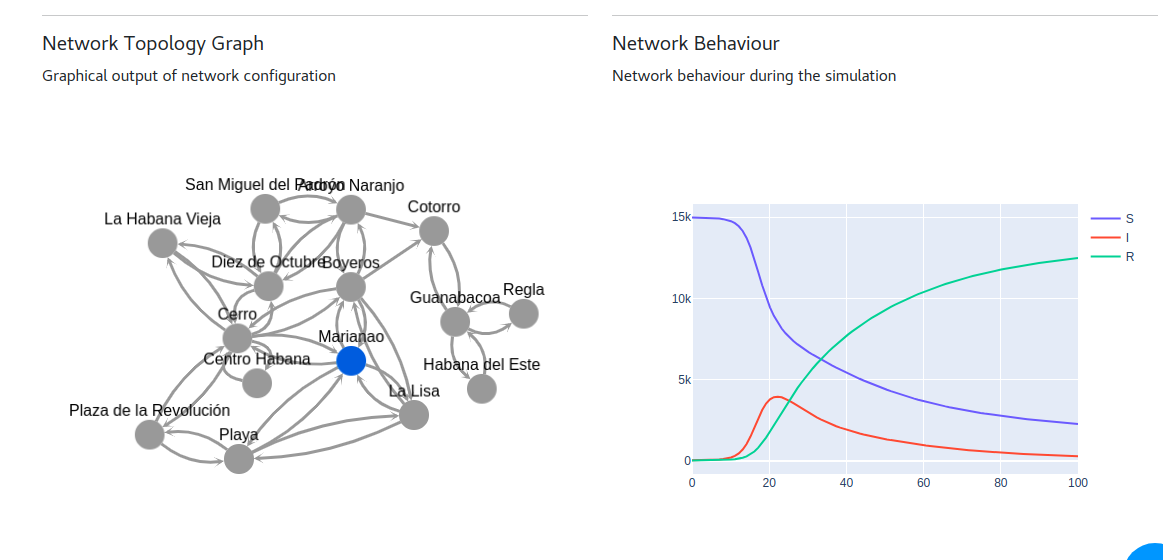
\includegraphics[width=0.9\linewidth]{./3}
	\caption{Gráficas}
	\label{Fig.3}
\end{figure}

Se muestra una representación gráfica de la red establecida y una gráfica que expone el comportamiento de la simulación.\\
Los nodos de la red pueden ser desplazads a conveniencia y al seleccionar uno de llos, se muestra su comportamiento (Fig.4).

\begin{figure}[H]
	\centering
	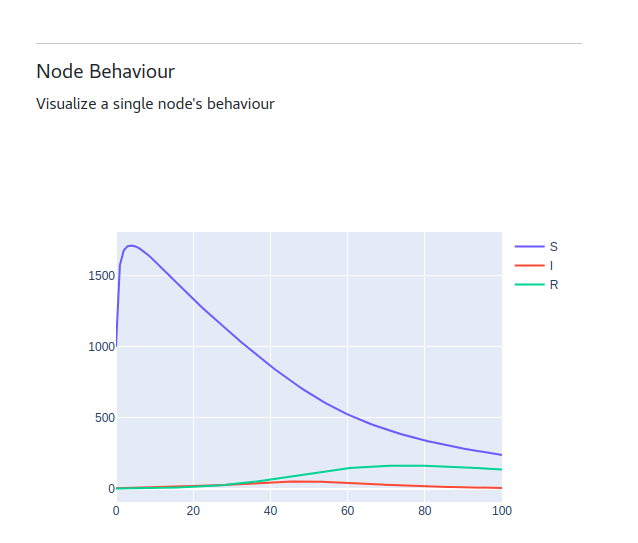
\includegraphics[width=0.9\linewidth]{./4}
	\caption{Nodo seleccionado}
	\label{Fig.4}
\end{figure}



\section*{Formato de redes a importar}
\subsection*{.json}
A continuación se muestra un ejemplo de red sencilla.
\begin{lstlisting}
{
	"graph": 
	{
		"directed" : false,
		"nodes" :
		 {
			"1" : 
				{
					"label" : "node1",
					"metadata" : {
					"cmodel" : "SIR"
				}
			},
			"2" : 
				{
					"label" : "node2",
					"metadata" : {
					"cmodel" : "SIR"
				}
			}
		},
		"edges": 
		[
			{
				"source" : "1",
				"target" : "2",
				"metadata" : {"weight" : 0.5}
			},
			{
				"source" : "2",
				"target" : "1",
				"metadata" : {"weight" : 0.5}
			}
		]
	}
}
\end{lstlisting}
Se siguen las especificaciones de formato de grafos que se muestran \href{https://jsongraphformat.info/}{aquí}.\\
Debe tener un objeto que tenga un objeto $graph$. Este último debe tener dos objetos, $nodes$ y $edges$.\\
En $nodes$ debe haber una serie de objetos cuyos nombres serán los $id's$ de cada nodo. Estos objetos tendrán un objeto $label$ cuyo valor es un string que representa el nombre del nodo. Además también tendrá un objeto $metadata$ que posee la información adicional necesaria (en este caso sólo es necesario $cmodel$ cuyo valor debe ser un string con el tipo de modelo).\\
En $edges$ se debe proporcionar una lista con las aristas de la red. Cada objeto de la lista tendrá un objeto $source$ y un objeto $target$ que deben tener los $id's$ del nodo fuente y destino respectivamente. En $metadata$ se debe tener un objeto $weight$ con el peso de la arista en cuestión cuyo valor debe ser un float.

\subsection*{.xml}
A continuación se muestra un ejemplo sencillo de una red con 3 nodos y dos aristas:

\begin{lstlisting}
<?xml version="1.0" encoding="UTF-8"?>
<graphml xmlns="http://graphml.graphdrawing.org/xmlns"  
    xmlns:xsi="http://www.w3.org/2001/XMLSchema-instance"
    xsi:schemaLocation="http://graphml.graphdrawing.org/xmlns
     http://graphml.graphdrawing.org/xmlns/1.0/graphml.xsd">
  <key id="d0" for="node" attr.name="cmodel" attr.type="string"/>
  <key id="d1" for="node" attr.name="label" attr.type="string"/>
  <key id="d2" for="edge" attr.name="weight" attr.type="double"/>
  <graph id="G" edgedefault="directed">
	  <node id="1">
		  <data key="d0">SIR</data>
		  <data key="d1">node1</data>
	  </node>
	  <node id="2">
		  <data key="d0">SIR</data>
		  <data key="d1">node2</data>
	  </node>
	  <node id="3">
		  <data key="d0">SIR</data>
		  <data key="d1">node3</data>
	  </node>
	<edge source="2" target="1"> <data key="d2">0.5</data></edge>
	<edge source="3" target="1"><data key="d2">0.5</data></edge>
  </graph>
</graphml>
\end{lstlisting}

El formato usado es \href{http://graphml.graphdrawing.org/}{GraphML}, el cual permite de una forma bastante flexible caracterizar  numerosos tipos de grafos. La primera línea del documento especifica la versión de XML y el encoding del documento. La segunda línea define la raíz del documento $graphml$. Este elemento como todos los demás pertenecen al $namespace$  http://graphml.graphdrawing.org/xmlns. A continuación siguen los atributos usados especifícamente para nuestro programa. El atributo $cmodel$ indica el tipo de modelo en el nodo y tiene $id=d0$. Para ponerles etiquetas a los nodos se usa el atributo $label$ cuyo $id=d1$. Finalmente, para especificar el peso de las aristas se usa $weight$ con $id=d2$.

Luego de esta sección viene la especificación del grafo. La misma está formada por dos elementos fundamentales: $node$ y $edge$. Como su nombre sugiere, $node$ representa un nodo de la red, al cual se le asigna un identificador y en los subelementos de tipo $data$ se les especifican sus atributos ( en este caso son una etiqueta y el modelo ). Para el caso de las aristas se usa el elemento $edge$, el cual tiene  que especificar un nodo origen y un nodo destino a través de los tags $source$ y $target$ respectivamente. Como mismo sucede en el caso de los nodos, los atributos ( en este caso es el peso de la arista solamente ) se especifican en el subelemento $data$. 

\section*{Formato de parámetros de entrada}
\subsection*{.json}
La plantilla generada tendrá la siguiente forma (se muestra un ejemplo básico).

\begin{lstlisting}
[
	{
		"id": "1",
		"label": "node1",
		"model": "SIR",
		"y": { "S": 999, "I": 1, "R": 0 },
		"params": { "beta": 0.2, "gamma": 0.1, "N": 1000 }
	},
	{
		"id": "2",
		"label": "node2",
		"model": "SIR",
		"y": { "S": 999, "I": 1, "R": 0 },
		"params": { "beta": 0.2, "gamma": 0.1, "N": 1000 }
	}
]
\end{lstlisting}
Cada objeto de la lista (lista de nodos) tendrá, además de sus objetos básicos, dos objetos $y$ y $params$. Estos tendrán a su vez una serie de objetos que representan los parámetros modificables de cada nodo. Cambie los valores de estos a conveniencia

\subsection*{.xml}
La plantilla generada tendrá la siguiente forma (se muestra un ejemplo básico).
\begin{lstlisting}
<nodes>
	<node1 id="1" label="node1" model="SIR">
		<y S="999" I="1" R="0"></y>
		<params beta="0.2" gamma="0.1" N="1000"></params>
	</node1>
		<node2 id="2" label="node2" model="SIR">
		<y S="999" I="1" R="0"></y>
	<params beta="0.2" gamma="0.1" N="1000"></params>
	</node2>
</nodes>
\end{lstlisting}
Similar al formato del .json. Modifique los atributos de los objetos $y$ y $params$ a conveniencia
\end{document}
